\section{UI-Komponenten ausblenden}
\label{hidingui-main}
Eine gute Möglichkeit, die Komplexität einer View zu verringern, ist das Ein- und Ausblenden von Komponenten. Teile, die für den Anwender aktuell nicht von Interesse sind, können bei Bedarf ein- oder ausgeblendet werden, wodurch sich die Übersichtlichkeit und Wahrnehmung für den Anwender verbessert. Gleichzeitig kann dies auch einen positiven Effekt auf die Performance haben. Denn je weniger Elemente sich im \gls{dom} befinden, desto schneller können Rendering-Prozesse durchgeführt werden. Siehe dazu Kapitel \ref{browser-engines}. 
\\\\
In AngularJS können \gls{ui}-Komponenten durch unterschiedliche Direktiven ein- oder ausgeblendet werden. Diese Direktiven unterscheiden sich anhand ihrer Funktionsweise und sind deshalb für unterschiedliche Einsatzzwecke geeignet. Die Direktiven \emph{ngShow} und \emph{ngHide} basieren darauf, abhängig von einer Bedingung über \gls{css}-Attribute einzelne \gls{html}-Elemente ein- oder auszublenden \cite{AJSNGIF}. Das \gls{css}-Attribut \emph{display} mit dem Wert \emph{none} blendet das Element aus, indem die Browser-Engine es nicht mit in den Render-Tree übernimmt \cite{hbw}. Im \gls{dom}-Tree bleibt es jedoch weiterhin bestehen. In Kombination mit AngularJS bedeutet dies, dass Models, Controller und Two-Way-Databindings auch nach dem Ausblenden weiterhin bestehen bleiben. Die Alternativen \emph{ngIf} und \emph{ngSwitch} basieren ebenfalls darauf, abhängig von einer Bedingung ein Element ein- oder auszublenden. Bei diesen Varianten wird das Element jedoch vollständig aus dem \gls{dom}-Tree entfernt \cite{AJSNGSHOW}.
\begin{figure}[h]
	\centering
	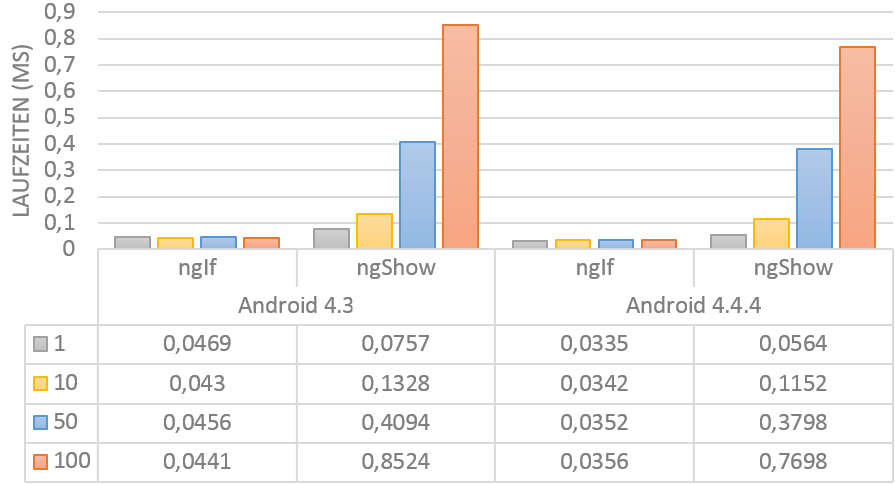
\includegraphics[scale=0.4]{Bilder/Diagramme/HidingUI-Digest.png}
	\caption{UI-Komponenten ausblenden - Laufzeitmessung \emph{\$digest}-Zyklus ngIf vs. ngShow}
	\label{hiding-ui-digest}
\end{figure}
Um die optimalen Einsatzzwecke beider Varianten zu ermitteln, werden zunächst verschiedene Tests hinsichtlich der Performance durchgeführt. Der erste Test prüft die Dauer des \emph{\$digest}-Zyklus, wenn das Element ausgeblendet ist. Der zweite Test misst die Zeit für das Einblenden und Ausblenden beider Varianten. Beide Tests werden mit einer Liste von Beispieldaten durchgeführt, deren Größe variiert. Abbildung \ref{hiding-ui-digest} zeigt das Ergebnis der Messungen des \$digest-Zyklus. Wie man dem Diagramm entnehmen kann, bleibt die Laufzeit unter Einsatz der Direktive \emph{ngIf} bei beiden Android Versionen unabhängig von der Anzahl der Elemente in der Beispielliste nahezu konstant. Diese Beobachtung lässt sich damit erklären, dass \gls{dom}-Elemente vollständig aus dem \gls{dom} entfernt und jegliche AngularJS Konstrukte beim Ausblenden durch \emph{ngIf} gelöscht werden. Bei \emph{ngShow} hingegen steigt die Laufzeit stetig mit der Anzahl an beobachteten Werten durch das Two-Way-Databinding an. Aus diesen Beobachtungen lässt sich schließen, dass \emph{ngIf} effektiver wird, je mehr Gebrauch die \gls{ui}-Komponente von Two-Way-Databindings macht. Im Vergleich der beiden Android Versionen zeigt sich auch hier, ähnlich wie in Abschnitt \ref{dv-analyse}, dass Android 4.4.4 hinsichtlich der reinen JavaScript Ausführung schneller ist. 
\\\\
Der zweite Test befasst sich mit der Performance des Ein- und Ausblendens von \gls{ui}-Komponenten. Abbildung \ref{hiding-ui-hideshow} zeigt die Ergebnisse dieses Tests. Es wird deutlich, dass \emph{ngShow} eine Komponente im Mittel 29\% schneller ein- bzw. ausblenden kann als \emph{ngIf}. Durch das Setzen des \gls{css}-Attributs \emph{display: none} werden \gls{ui}-Komponenten lediglich im Rendering-Prozess nicht berücksichtigt. Der Zugriff auf den \gls{dom} wird im Gegensatz zu \emph{ngIf} eingespart. Im Vergleich zwischen Android 4.3 und Android 4.4.4 zeigt sich, dass Android 4.3 im Mittel 212\% schneller ist. Allgemein lässt sich aus diesen Ergebnissen schließen, dass \emph{ngShow} effektiver wird, je öfter eine \gls{ui}-Komponente ein- bzw. ausgeblendet werden soll. 
\begin{figure}[h]
	\centering
	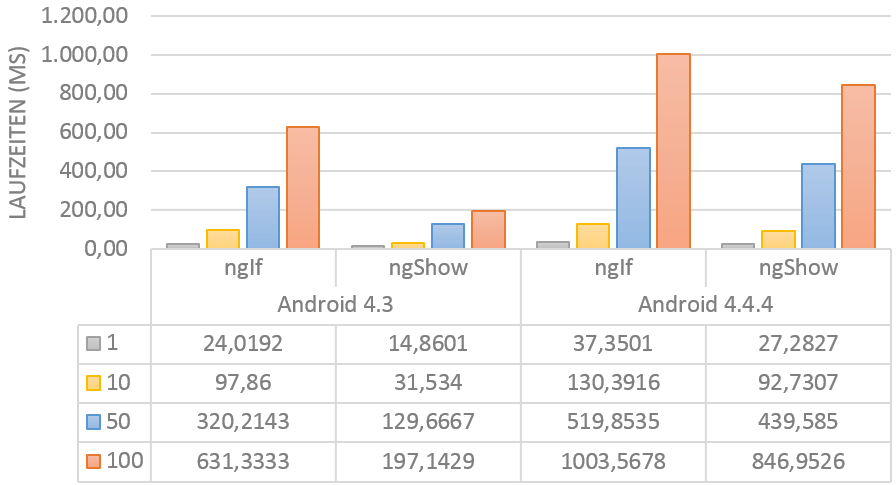
\includegraphics[scale=0.4]{Bilder/Diagramme/HidingUI-ShowHide.png}
	\caption{UI-Komponenten ausblenden - Laufzeitmessung Ein-/Ausblenden ngIf vs. ngShow}
	\label{hiding-ui-hideshow}
\end{figure}